



\setlength{\tabcolsep}{2pt}  % Tighter spacing for multi-level table


\begin{table*}[t]
\vspace{-2mm}
\centering
\scriptsize
% \caption{Comparison of framework categories, covering agent structure, multi-agent interaction, and environment modeling.}

\caption{Our taxonomy of multi-agent LLM frameworks, organizing frameworks by architectural paradigms and design dimensions.}
\vspace{-3mm}
\label{tab:framework-comparison}
\renewcommand{\arraystretch}{0.9}
\begin{tabular}{
    m{3.2cm}%
    >{\centering\arraybackslash}m{4.6cm}%
    >{\centering\arraybackslash}m{4.6cm}%
    >{\centering\arraybackslash}m{4.6cm}%
}
\toprule
\textbf{Feature} & \textbf{Graph-Based (LangGraph)} & \textbf{Role-Based (CrewAI)} & \textbf{GABM (Concordia)} \\
\midrule

\multicolumn{4}{l}{\textbf{1. Single-Agent Characteristics}} \\

\quad Main Purpose 
    & Deterministic workflow orchestration via explicit execution graphs; agent-based 
    & Task-driven coordination via role-specialized agents and delegation; task-based
    & Simulation of emergent behavior through environment-mediated agent interaction \\

\quad Agent Architecture
    & \parbox[c]{\linewidth}{\centering
        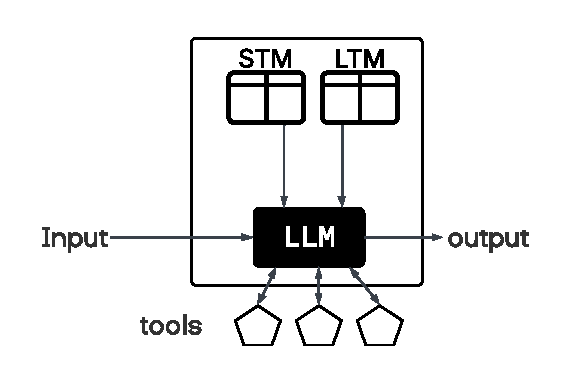
\includegraphics[width=.85\linewidth, trim=.4cm .4cm .4cm .4cm, clip]{figures/langraph-single-agent3.pdf}}
    & \parbox[c]{\linewidth}{\centering
        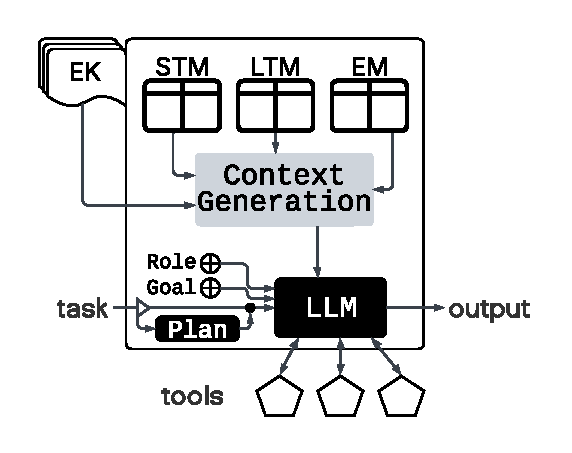
\includegraphics[width=.85\linewidth, trim=.5cm .5cm .5cm .5cm, clip]{figures/crewAI-single-agent2.pdf}}
    & \parbox[c]{\linewidth}{\centering
        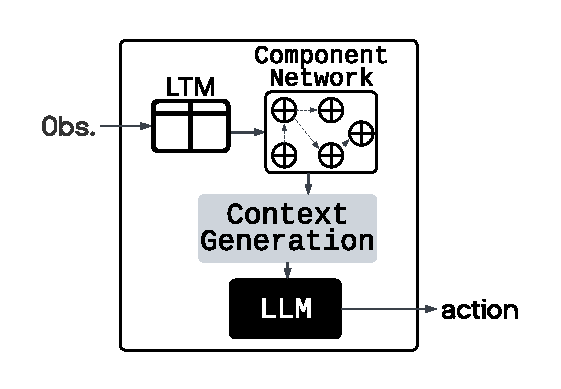
\includegraphics[width=.85\linewidth, trim=.4cm .4cm .4cm .4cm, clip]{figures/Concordia-single-agent2.pdf}} \\


\multicolumn{4}{l}{\textbf{\quad Behavioral Specification}} \\

\quad\quad Role 
    & \xmark~Implicit; No first-class role abstraction 
    & \checkmark~Explicit; First-class role abstraction 
    & \checkmark~Optional; Provided class targets social experiments \\

\quad\quad Goal %(what “success” looks like)
    & \xmark~Determined by graph; No first-class goal object 
    & \checkmark~First-class object; fixed; one per agent
    & \xmark~Environment-driven; No first-class goal object \\

\quad\quad Planning 
    & \xmark~Embedded in graph; LLM planning requires coding 
    & \checkmark~Pre-task or manager-worker planning
    & \checkmark~Optional; Provided class targets social experiments \\




\multicolumn{4}{l}{\textbf{\quad Storage}} \\

\quad\quad Long-Term Memory (LTM) 
    & \checkmark~ Retrieval-based semantic store 
    & \checkmark~Retrieval-based semantic store
    & \checkmark~LLM-queried textual memory \\

\quad\quad Short-Term Memory (STM) 
    & \checkmark Conversation or state accumulation within execution  
    & \checkmark~RAG-based working context over recent interactions 
    & \xmark~Not natively supported \\

\quad\quad Entity Memory (EM)
    & \xmark~Not natively supported 
    & \checkmark~Optional; structured entity facts via retrieval
    & \xmark~Not natively supported \\

\quad\quad Working Memory (WM)
    & \xmark~State variables must be managed by developer
    & \xmark~Implicit via task context; not explicitly modeled 
    & \checkmark~Derived from LTM; update rules by developer \\

\quad\quad External Knowledge (EK)
    & \xmark~Not natively supported 
    & \checkmark~Explicitly attachable (files, strings)   
    & \xmark~Not natively supported \\



\textbf{\quad Tool Execution}
    & \checkmark~Agent-bound tools or explicit graph tool nodes  
    & \checkmark~Agent-bound tools
    & \checkmark~Tools executed by environment, not by agents \\

    
\midrule

\multicolumn{4}{l}{\textbf{2. Multi-Agent Characteristics}} \\

\quad Network Topology 
    & \parbox[c]{\linewidth}{\centering
        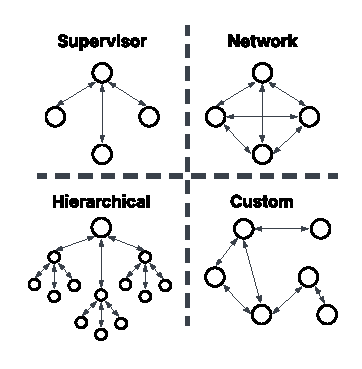
\includegraphics[width=.7\linewidth, trim=.48cm .48cm .4cm .6cm, clip]{figures/Graph-Based-Topology.pdf}}
    & \parbox[c]{\linewidth}{\centering
        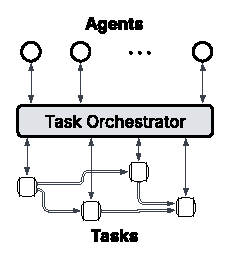
\includegraphics[width=.45\linewidth, trim=.28cm .23cm .2cm .3cm, clip]{figures/crewAI-multi-agent.pdf}}
    & \parbox[c]{\linewidth}{\centering
        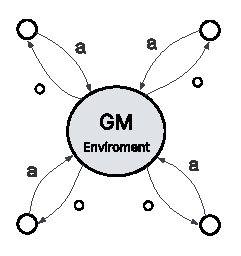
\includegraphics[width=.5\linewidth, trim=.28cm .28cm .2cm .3cm, clip]{figures/GABM-Based-Topology.pdf}} \\

\quad  
    & \checkmark~Flexible; fixed once defined
    & \checkmark~Task hierarchy or sequence 
    & \checkmark~Fixed star topology; GM at center \\

\quad Communication Pattern 
    & \checkmark~Shared state along predefined edges 
    & \checkmark~Task-mediated; limited peer querying 
    & \xmark~Only via GM; no peer-to-peer \\

\quad Collaboration 
    & \xmark~None; procedural coordination only 
    & \checkmark~Partial; delegation-based coordination only 
    & \xmark~None; no explicit collaboration mechanisms \\

\midrule

\multicolumn{4}{l}{\textbf{3. Environment}} \\

\quad World State and Grounded Variables 
    & \xmark~None; execution context only 
    & \xmark~None; task-centric context only 
    & \checkmark~Explicit world state with grounded variables \\

\bottomrule
\end{tabular}
\vspace{-1mm}
\end{table*}
